\chapter{Pilot User Study Results And Analysis} \label{sec:results}

\section{Participant Background Feedback}

\begin{figure}[h]
	\centering
	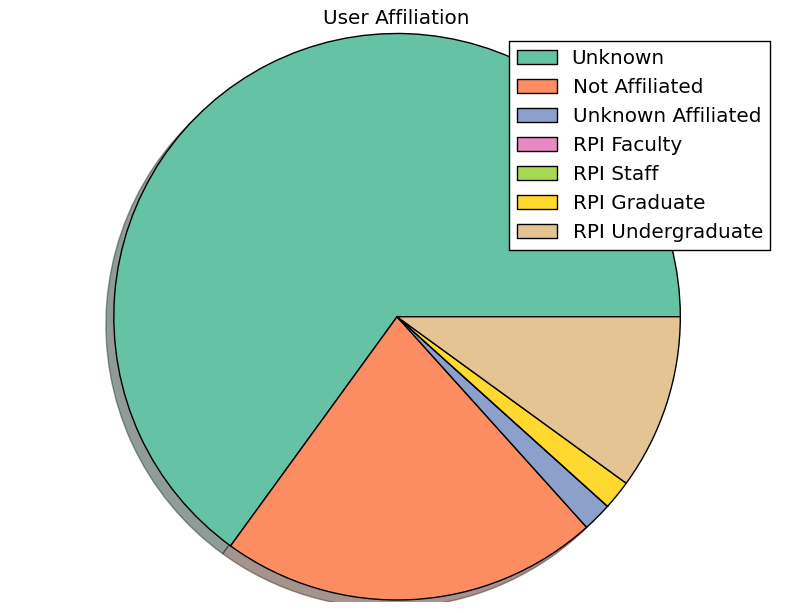
\includegraphics[width=0.8\textwidth]{rpi_affilation}
	\caption{User affiliations of participants on OASIS}
	\label{fig:rpi_affilation}
\end{figure}

In the two week timespan that OASIS was publicly available 57 users registered and participated in our pilot user study.
I recruited participants for our pilot user study on large social media outlets such as Facebook and Reddit.
Both of these social media outlets have a wide range of users with varying experiences.
Not to mention, one of the online outlets I recruited participants from is unofficially affiliated with Rensselaer Polytechnic Institute (RPI). 
Figure-\ref{fig:rpi_affilation} demonstrates the affiliation of participants who registered on OASIS.
As shown in Figure-\ref{fig:rpi_affilation} a majority of participants that provided their affiliation are not affiliated with RPI. 
This is a big change from previous user studies, where all the participants were RPI affiliated.
Additionally, Figure-\ref{fig:rpi_affilation} shows that the majority of participants that are affiliated with Rensselaer Polytechnic Institute, are undergraduate.
It is also interesting that the majority of participants choose not to provide information on their affiliation with RPI.
Specifically, 65\% of participants did not provide feedback on their affiliation, and not all participants who claimed to be affiliated with RPI specified how they were affiliated;
About 2\% of participants have unknown affiliations with RPI.
The difference between RPI affiliated participants and non-RPI affiliated participants could be a direct results of how and when we recruited participants for the pilot user study.
During the pilot user study we advertised towards non-RPI affiliated social media outlets first and  RPI affiliated social media outlets last. 
There was more time recruit non-RPI affiliated participants than RPI affiliated participants. \\

\begin{figure}[h]
	\centering
	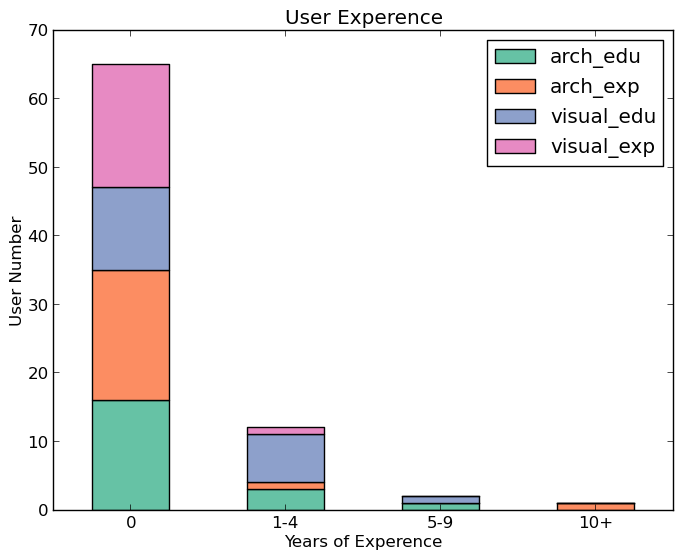
\includegraphics[width=0.8\textwidth]{exp_edu}
	\caption{Architecture and visual arts experience of OASIS participants }
	\label{fig:exp_edu}
\end{figure}

Similarly, I asked our participants about their experience with architecture and visual arts.
Figure-\ref{fig:exp_edu} shows the distribution of participants' formal education and job experience in both fields of architecture and visual arts.
A majority of our participants expressed that they have no experience with any of the related fields;
As a result, these participants will be referred to as non-experts.
Also a majority of those participants that have experience, generally have only 1-4 years of exposure to formal architecture education or form visual arts education.
However, there is one user registered on OASIS that claims to have over 10 years of job experience in architecture.
Aside from asking about architecture and visual arts experience, I also let participants elaborate on other relevant experiences. 
Some of our participants have had experience in civil engineering, electrical engineering, studio arts, user experience design, and architectural engineering with focus in lighting.
While our current set of participants does not have much experience with architecture, they do encompass a board range of related fields.\\

\begin{figure}[h]
	\centering
	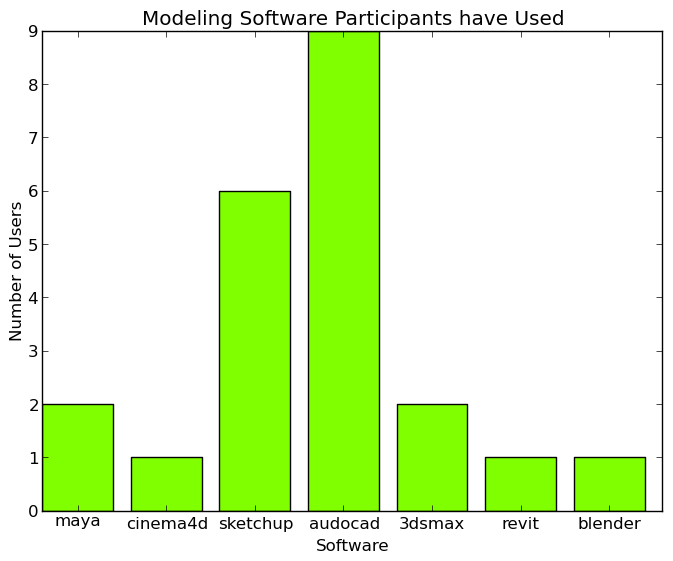
\includegraphics[width=0.8\textwidth]{software_exp}
	\caption{Participants' experience with 3D Modeling Softwares}
	\label{fig:software_exp}
\end{figure}


Furthermore, I also asked participants to provide a list of 3D modeling software they have had exposure to.
As seen in Figure-\ref{fig:software_exp} participants have had the most experience with AudoCad\cite{} and SketchUp\cite{}. 
A few participants have had experience with 3dsMax\cite{} and Maya\cite{}.
Again, we let participants elaborate on their experience with other 3D modeling software. 
Other 3D modeling software, not shown in Figure-\ref{fig:software_exp}, that participants have had experience using include SolidWorks\cite{}, AGI32\cite{}, Dialux\cite{}, and Daysim\cite{}.
Note that AGI32, Dialux, and Daysim are not specifically 3D modeling tools but rather used for daylight analysis and performance.
From user feedback collected in our pilot user study on participants' affiliations, experience in related fields, and exposure to modeling software, determine that OASIS is accessible to a wide variety of users. \\

\begin{figure}[h]
	\centering
	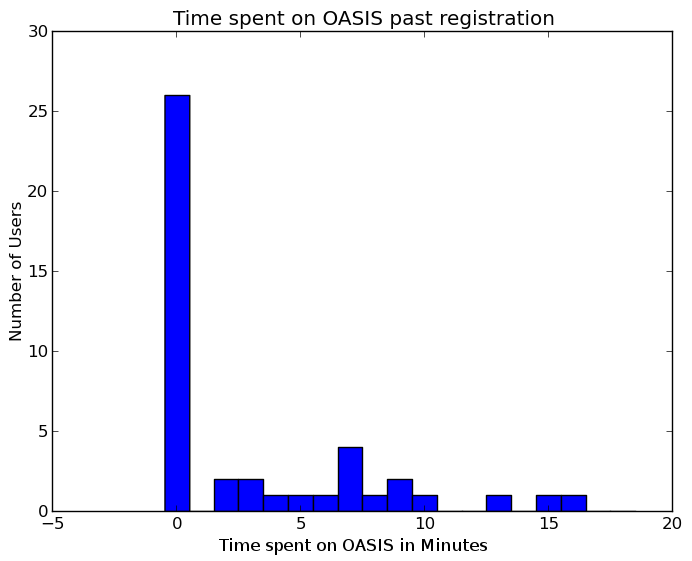
\includegraphics[width=0.8\textwidth]{time_oasis_hist}
	\caption{Distribution of time spent on OASIS per user}
	\label{fig:time_oasis_hist}
\end{figure}

In addition to trying understand if OASIS is accessible, I also wanted feedback on the usability.
Analyzing data on how participants spend time their on OASIS can provide insight on user behavior.
Figure-\ref{fig:time_oasis_hist} illustrates the distribution of participants in relation to their time spend on OASIS.
From Figure-\ref{fig:time_oasis_hist} is it clear that the majority of users registered and participating in the pilot user study spent no time on the actual interface.
On the other hand, the average time spent per participant is about 12 minutes, excluding participants that do not spend longer than a minute on OASIS past registration.
Although our user retention rate is low, I suspect that the voluntary nature, anonymity, and absence of renumeration in our pilot user study plays a significant role in the large number of participants who register and do not use OASIS.

\begin{figure}[h]
	\centering
	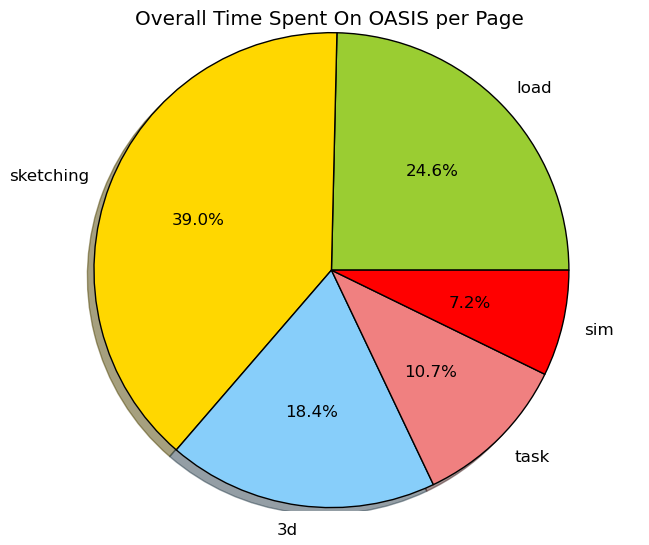
\includegraphics[width=0.8\textwidth]{time_chart}
	\caption{Breakdown of time spent on OASIS pages}
	\label{fig:time_chart}
\end{figure}

Furthermore, we have no data on user participation in similar online user studies targeting similar social media outlets.
Equally important, Figure-\ref{fig:time_chart} illustrates participant time spend on OASIS per page.
Moreover, Figure-\ref{fig:time_chart} shows that participants spend 36\% of their time on the \textit{ Sketch a Room} page.
Next participants spend 23\% of their time on the \textit{Create/Load Model}page.
It is important to note that first-time users have the option of viewing a short tutorial video; 
the 1 minute long tutorial video coupled with redirection to the \textit{Create/Load Model} page after logging in, could directly contribute to the large portion of time participants spend on the \textit{Create/Load model} page.
Surprisingly, the page participants spend the least amount of time is on the \textit{Analyze Simulation} page. 
On the \textit{Analyze Simulation} page user can view daylight renderings of user designed models.
On average participants spent only 8\% of their time analyzing their designed models;
when compared to the 25\% of time participants spend on viewing 3D interpretations on the \textit{Generate 3D model} page, the time spend on the \textit{Analyze Simulation} page seems remarkably low.
The difference between time spend on these two pages could stem from the fact that the \textit{Analyze Simulation} page is the final page new users visit when navigating OASIS linearly.
Furthermore, all of the temporal data collected on pages in OASIS could be effected by time spend writing feedback questions, multi-tasking while leaving OASIS running in the background, and leaving OASIS before visiting all pages.
 
\section{Usability Feedback}

\begin{table}[h]
\centering
\begin{tabular}{|p{0.2\textwidth}|p{0.8\textwidth}|}
\hline
\rowcolor[HTML]{EFEFEF} 
{\color[HTML]{000000} \textbf{Username}} & {\color[HTML]{000000} \textbf{Response}} \\ \hline
galarodo & The beds/desks/wardrobes are good images and helpful when determining the scale \\ \hline
dcheung3 & Creating the structure was interesting \\ \hline
damamani & The objects have very easy buttons to adjust orientation and position. This app is great for arranging new apartments to visualize where to get sunlight \\ \hline
kyoko.usagi & Kind {[}of{]} like the skylight option to be honest \\ \hline
mike smith & the furniture \\ \hline
tranthang & you can customize the room and have the light orientation \\ \hline
Solyha & It took me a few tries to get the windows in. I didn't realize you had to put a wall in and the window on top of that. I was leaving a space for the window. \\ \hline
Jan Selz & It was easy to understand the intent but a challenge to work with limited options. \\ \hline
ktran101 & This was fun. Definitely interesting \\ \hline
durkeejw & Very simple, never ran into a ``you can't do this'' \\ \hline
flowerJane & It's really easy to figure out how to use the features. \\ \hline
mindykay & I find this tool extremely convenient to use and it`s really fun to sketch new designs for future interior design plans! \\ \hline
qjkxkcd & It's very easy to use. The interface is very intuitive. \\ \hline
alanlang & the day-lighting simulation \\ \hline
\end{tabular}
\caption{Feedback to the question: What did you find fun or interesting in this sketching environment?}
\label{fig:fun}
\end{table}

Most of the feedback collected on the usability of OASIS is qualitative.
Quantitative boolean feedback would not fully capture how participants are experiencing our sketching interface;
As a result, I collect qualitative feedback to gain insight into how users perceive OASIS.
Table-\ref{fig:fun} list feedback collected from 14 participants concerning what participants found fun or interesting in our sketching environment.
Overall, 6 of the participants mentioned that the interface was either fun or easy-to-use.
However, some participants found window placement non-intuitive; 
other participants had difficulty with the limited primitives we provide.
While, we did not explicitly ask what they found difficult difficult in the interface in this specific feedback question, their response will be taken into consideration.
The participant who found window placement difficult states that they tried to ``leave a gap between walls to define where to place windows''.
I suspect that the participant, with this issue, must have skipped the tutorial video or not consulted the any of the help options on OASIS.
By the same token the other participant, concerned with the limited options on OASIS, I speculate is comparing our tool to other more fully featured modeling softwares.
As stated before, we intent for OASIS to be an early design tool for use during the schematic design phase of architecture.
As a result, for the pilot study I did not prioritize our selection of furniture items, but choose a three pieces of furniture found commonly in bedrooms.
Interestingly, our only participant with over 10 years of architectural job experience stated that the sketching interface was ``very simple'' and that that they never encountered modeled that could not be interpreted.
Other participants claim they find specific features interesting, including the furniture items we support, skylights, and the daylight simulations.\\


\begin{table}[h]
\centering

\begin{tabular}{|p{0.2\textwidth}|p{0.8\textwidth}|}
\hline
\rowcolor[HTML]{EFEFEF} 
Username   & Response                                                                                                                                                                                       \\ \hline
dcheung3   & Addition of precise measurements of the walls and windows would be good. Have more options on items besides desk and wardrobe. Be able to distinguish between open entrance ways and doorways. \\ \hline
Jan Selz   & I only see items to create a bedroom.  There should be additional items to create other types of rooms.  It was also uncomfortable, not to be able to place a door.                            \\ \hline
ktran101   & Maybe there can be more options for other pieces of furniture? Or just blocks that can represent it.                                                                                           \\ \hline
durkeejw   & Window size, ceiling height, window surface finishes                                                                                                                                           \\ \hline
flowerJane & Change the width and height of furniture, click and drag the walls                                                                                                                             \\ \hline
mindykay   & Possibly adding the ability to install doors!                                                                                                                                                  \\ \hline
\end{tabular}
\caption{Feedback to the question: What additional features should be added to the system to allow greater flexibility in design?}
\label{fig:features}
\end{table}

We also asked participants to provide additional features we could add to our sketching interface to extend the flexibility of OASIS.
The two of the most common features requested by participants are the addition of doors on the sketching interface and a wider variety of furniture items.
Also, some participates desired more control over primitives on the sketching interface. 
Including both drag and drop mechanics on walls after initial placement and the precise manipulation of furniture dimensions.
Additionally, our sole participant with over 10 years or architecture experience suggest we offer control over window heights, ceiling heights, and window finishes.
These features are most commonly found in daylighting analysis software and are features important if I plan to define OASIS as a tool for daylighting analysis.
Interestingly, an unanticipated situation with participants' feedback was discovered when analyzing the feedback for this question.
A few of our 14 participants provided duplicate responses from previously asked questions.
Table-\ref{fig:features} displays  all responses collected that were not duplicate responses to previous questions. \\
 

\begin{table}[h]
\centering
\begin{tabular}{|p{0.2\textwidth}|p{0.8\textwidth}|}
\hline
\rowcolor[HTML]{EFEFEF} 
\textbf{Username} & \textbf{Response} \\ \hline
galarodo & Lofted beds with desks underneath \\ \hline
dcheung3 & Doors for enclosement \\ \hline
ryasoa & Add television and couch \\ \hline
damamani & I'd like to be able to connect the walls together and select all of them. I didn't have the ability to scale the objects.  I also would've like to have the ability to move the walls around. There is no undo button or keyboard shortcut. \\ \hline
kyoko.usagi & No doorway, kinda important + furniture options kinda would help create the ambiance \\ \hline
mike smith & multiple rooms \\ \hline
tranthang & circular designs \\ \hline
Solyha & I would like to put in the items that hang on the wall to see how long they might be in direct sunlight. \\ \hline
Jan Selz &  \\ \hline
ktran101 & perhaps more furniture options. \\ \hline
durkeejw & Light shelves \\ \hline
mindykay & I was not able to make more than one room, since I can`t put int a door. \\ \hline
qjkxkcd & Reflective surfaces would add to a model's accuracy (e.g. glass/mirror/water). But maybe those are beyond the scope of this tool. \\ \hline
\end{tabular}
\caption{Feedback to the question: Describe some designs that you were not able to create due  to system limitations. }
\label{fig:limitation}
\end{table}

In addition to collecting feature request feedback, I also ask participants to describe some designs that they were unable to create due to system limitations.
Table-\ref{fig:limitation} shows participants feedback on limitations of design in our sketching interface.
The most common design limitation observed was the absence of doors in our sketching interface.
From the feedback collected, it seems that participants assumed that they could not design multi-room sketches because of the lack of doors in the sketching interface.
In actuality, previous user studies have confirmed that the physical sketch interpretation algorithm can handle multi-room designs\cite{}.
Other design limitations participants claimed to face included the lack of light shelves in our interface, the inability to place one piece of furniture on top of another, and unavailability of control over scale.
Again, participants also expressed that our selection of furniture items limited designs. \\


\begin{table}[h]
\centering
\begin{tabular}{|p{0.2\textwidth}|p{0.8\textwidth}|}
\hline
\rowcolor[HTML]{EFEFEF} 
\textbf{Username} & \textbf{Response} \\ \hline
dcheung3 & There wasn't any real-time measurements when making the walls and windows that would have been beneficial in capturing more accurate model. \\ \hline
damamani & I'd like more objects. \\ \hline
kyoko.usagi & no doors {[}equal{]} not proud \\ \hline
mike smith & nope \\ \hline
tranthang & Cant move the walls \\ \hline
Solyha & I would like a graph in the background so that I could be more accurate with the dimensions. \\ \hline
Jan Selz & I have a Building Information Modeling program open in the background.,I kept wanting to use commands and shortcuts for that program and it was difficult to simply just draw.,(more personal issue than program issue) \\ \hline
mindykay & Nope! \\ \hline
qjkxkcd & The location selector could be easier to use accurately but I guess it's not really important. An ``undo'' feature might be handy also. \\ \hline
\end{tabular}
\caption{Feedback to the question: Was there anything you did not like about working in this sketching environment?}
\label{fig:dislike}
\end{table}

Overall, the main take away from participant feedback concerning design limitations is that doors are essential to communicate to users that our sketching interface supports multi room designs.
On a similar note Table-\ref{fig:dislike} list out participant feedback regarding disliked elements of our sketching interface.
A common dislike in our sketching interface was the absence of scale.
Currently, we convey scale indirectly though statically sized furniture items, however feedback suggest that we make scale more explicit to users.
Interestingly, a participant expressed dislike with our interface because we do not support keyboard shortcuts for common actions, such as undo.
Other dislikes with our sketching interface include the limited collection of furniture we support, absence of doors, the inability to move walls after initial placement, and the the lack of accurately when selecting a geographical locations for sketches.\\

\begin{table}[h]
\centering
\begin{tabular}{|p{0.2\textwidth}|p{0.8\textwidth}|}
\hline
\rowcolor[HTML]{EFEFEF} 
\textbf{Username} & \textbf{Response} \\ \hline
galarodo & Nope \\ \hline
dcheung3 & No, everything was very straight forward and user-friendly. \\ \hline
damamani & No,The user interface is very simple and easy. \\ \hline
kyoko.usagi & at first I couldn't put the walls in like I was stuck in the confine space of the circle, but I know that I would make it bigger. But I got the hang of it I guess \\ \hline
mike smith & nope \\ \hline
tranthang & N/A \\ \hline
Solyha & At first the ``buttons'' would not stay highlighted so I did not know if I was in the right mode at first. I wish you could move an item like the desk after it is placed to refine its location. I had to delete it and them put another one in when I was trying it out. \\ \hline
Jan Selz & It is very intuitive. \\ \hline
durkeejw & no, very easy \\ \hline
mindykay & None! \\ \hline
qjkxkcd & Were (typo in the question) + Apparently walls can be removed with the ``Remove'' operation, but it seems like furniture can't be + Also, when furniture is added, there are 3 white points that can be used to manipulate it; the center one controls the position, and both of the others rotate the object. Is one meant to resize it? Or are they supposed to do the same thing \\ \hline
\end{tabular}
\caption{Feedback to the question: Where there any elements of the user interface that were hard to use or confusing?}
\label{fig:hard2use}
\end{table}


Lastly, we asked participants if there were any elements in our interface that were hard to use.
Feedback from that question can be seen on Table-\ref{fig:hard2use}.
Many participant responded to this question with stating nothing was hard to use on OASIS.
However, a few users experienced software bugs with the interface and used this feedback question as a means to report them to us.
Aside from a few fixable software bugs, of which did not impact the entire system, a participant found the redundancy of Raphael FreeTransform handles confusing.
FreeTransform handles are three white circles that are overlaid onto furniture items when clicked in our sketching interface.
One circle appears at the center of the furniture item, and the two other circles are paced perpendicularly some distance away from the furniture item, as illustrated in Figure-\ref{fig:oldvh}F.
As of now, these two perpendicular handles are used solely to rotate items.
Participant feedback help us note overlooked redundancies in our interface such as two rotation FreeTransform handles that perform the same action.\\

To completely analyze the feedback collected from our sketching interface we must understand that omission of feedback could potentially be used to communicate feedback.
For example, when asked about negative aspects of our interface many users choose to respond with ``no'' or ``none''.
However, some participants, whom readily provide feedback, may decide to omit feedback for specific questions to communicate an implied ``no''.
Ambiguous omissions of feedback proses a problem for analysis. 
For example I cannot assume that users imply there are no negative elements on our sketching interface based on user omission of specific feedback questions, although participants may intentionally omitted feedback.
Improvements in how I collect participant feedback need be made to remove ambiguity in omitting feedback.
On a similar note, participants' feedback sometimes does not directly answer corresponding questions asks.
Occasionally, participants' feedback would be more appropriate as the response to another question.
I suspect that participants do no revise feedback after submitting and as a result some of our responses seem similar for multiple questions. \\

Despite all of this, the sketching interface garnered overall positive feedback from our participants.
Many participants, especially the non-experts, claimed that the interface was easy to use and interesting.
 
\section{Model Based Feedback}

\begin{figure}[h]
	\centering
	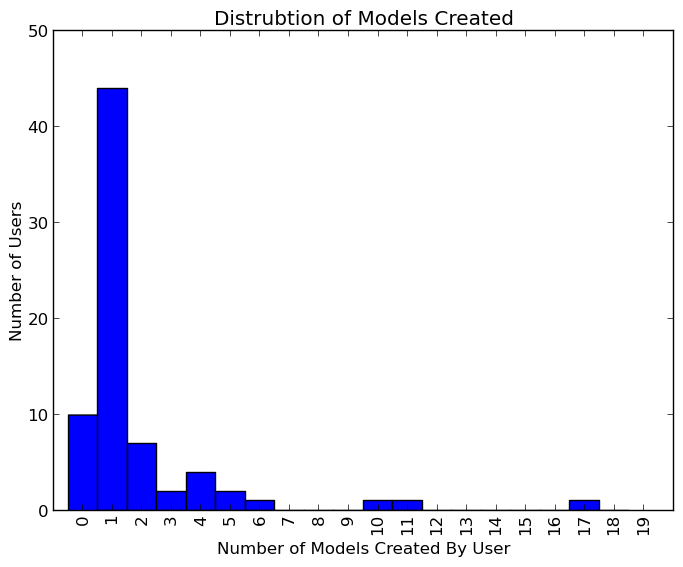
\includegraphics[width=0.8\textwidth]{model_hist}
	\caption{The distribution of models created on OASIS}
	\label{fig:model_hist}
\end{figure}


\begin{figure}[h]
	\centering
	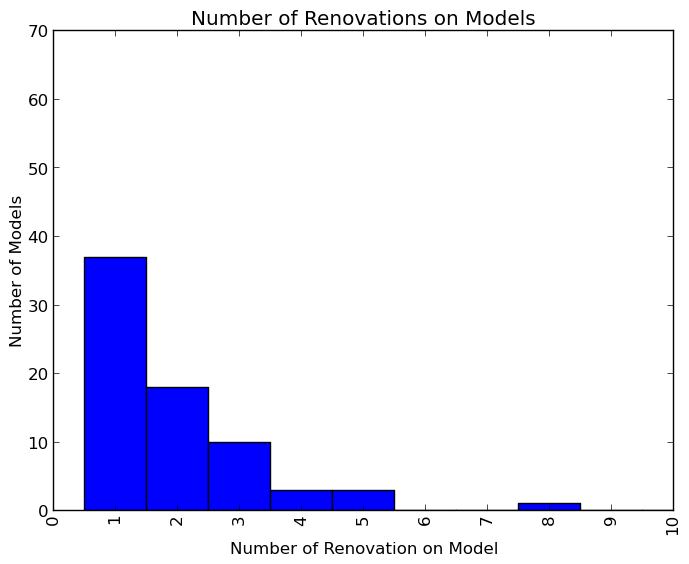
\includegraphics[width=0.8\textwidth]{renvo_hist}
	\caption{The distribution of renovations created on OASIS}
	\label{fig:renvo_hist}
\end{figure}

There are currently 73 models on OASIS and on average each user generates 1.25 models.
The distribution of the number of models made per user is illustrated in Figure-\ref{fig:model_hist}.
From Figure-\ref{fig:model_hist} we can see that most of our participant only crated a single model.
A handful of participants, however, created more than 9 models on our interface.
While the number of models per users is relatively low, the number of renovations per models show that on average there are 1.9 renovations per model created.
Meaning that about half of our participants renovate their models at least more than once.
Figure-\ref{fig:renvo_hist} show the distribution of models and the number of renovations on % these models.
Analysis of individual models is out of the scope of this thesis, however, I do display some user created models in Figure-\ref{fig:examples}. \\

\begin{figure}[h]
	\centering
	
\includegraphics[width=0.5\textwidth]{place_holder}
	\caption{Examples of some users created models on OASIS}
	\label{fig:examples}
\end{figure}

\begin{figure}[h]
	\centering
	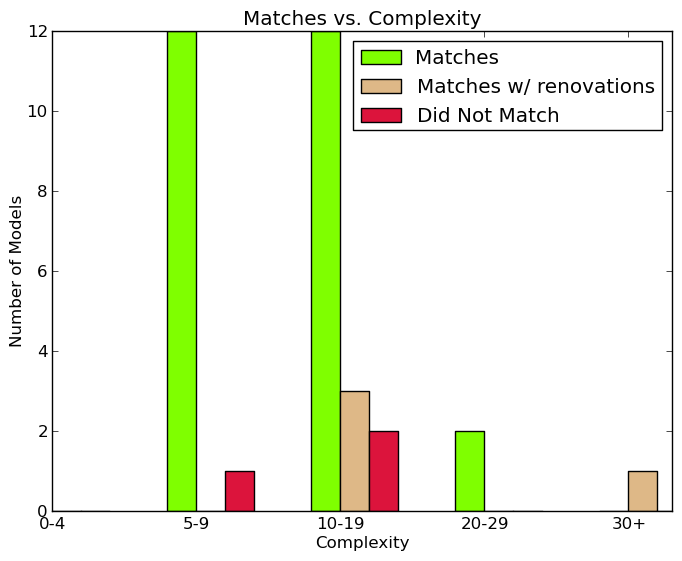
\includegraphics[width=0.8\textwidth]{matching_chart}
	\caption{Accuracy in relation to model complexity}
	\label{fig:matching_chart}
\end{figure}

After creating a 3D model participants can voluntarily provide feedback concerning the accuracy of our interpretation.
Participants can state the interpretation of their sketches were either a initially matched their intentions, a match after a performing adjustments as renovations, or not a match at all.
I hypothesized that as models grew more complex the accuracy of our interpretation algorithm would decrease.
Figure-\ref{fig:matching_chart} illustrates model complexity in relation to matching user intentions.
Model complexity is the sum of the number of primitives in a sketch.
Figure-\ref{fig:matching_chart} is interesting because models regardless of complexity seem to always match users initial intentions without requiring renovations.
Even models with 20 to 29 primitives seem to always match.
While the data is strongly indicative that our physical sketch interpretation algorithm is accurate, I believe that more feedback is required before any statically significant conclusions can be drawn.
From Figure-\ref{fig:matching_chart} and the fact that there are 73 models on OASIS, but only fewer responses makes it is clear that participants do not answer this specific feedback question readily.
In order to better gauge our accuracy, changes to the interface need to be made to persuade participants to answer this feedback question. \\


\begin{table}[h]
\centering
\begin{tabular}{|p{0.2\textwidth}|p{0.8\textwidth}|}
\hline
\rowcolor[HTML]{EFEFEF} 
\textbf{Username} & \textbf{Feedback} \\ \hline
qq & Can't make doors. Walls seem slanted in model visualization, which is probably intended. \\ \hline
Solyha & I still only see 2D \\ \hline
durkeejw & good, easy, fast \\ \hline
qjkxkcd & Model matched 2d representation from step 2. There was kind of a funky rendering issue (http://imgur.com/COBtYgv). (This was resolved when I remembered to add a final wall to close the room) + Also, when typing in this text box, using the arrow keys to navigate around text also pans the image around. \\ \hline
flowerJane & It was really fast and it rendered nicely \\ \hline
Jan Selz & Proportions of items and volume created seem to match the design intent. \\ \hline
mike smith & the program does a good job constructing the 3D model \\ \hline
ryasoa & It worked very well \\ \hline
damamani & Very good 3-D modeling but Step two needs some additional features to connect the walls properly. \\ \hline
principealberto & It is \\ \hline
tranthang & It well windows and furniture it is place windows fine \\ \hline
dcheung3 & Overall the 3D model does capture my sketch \\ \hline
alanlang & the 3D match my design \\ \hline
mindykay & This is really amazing! The 3D design is exactly what I was aiming for! \\ \hline
kyoko.usagi & I mean yes this kind of matches, but no doors is not in my intended design. That's why it failed. But the effectiveness is pretty spot on \\ \hline
galarodo & Accurate to the design.  Room was little bit wider (beds further apart) but requires to many edits to fix.  Deleting walls and redrawing them \\ \hline
\end{tabular}
\caption{Feedback to the question: Describe your overall impression of the system's effectiveness in constructing a 3D model from your design.}
\label{fig:effective}
\end{table}

Aside from categorical quantitative feedback, we also ask participants to quantitatively describe their overall impressions of the system's effectiveness in construction 3D models from user sketches; 
Table-\ref{fig:effective} displays results from this feedback questions.
Of the 16 participants that provided feedback on the effectiveness of the physical sketch interpretation algorithm, 14 stated that the system generally matched their intentions.
One participant stated that they only saw 2D versions of the interpretation.
I presume this could be caused from the user either not rotating their model or limited WebGL support on their web browser.
I do  not collect meta data on participants' web browsers or cursor movements, so currently there is no explanation of problem encountered by this participant.
Two participants mentioned the lack of support for doors hindered the effectiveness of generating 3D models.
One participant linked us an image in their feedback, that displayed a rendering issue they had encountered.
The detail of some of the qualitative feedback provided from participants was higher than originally expected.
A take away from participants taking screen shots, hosting images online, and linking images of problem renderings to us is that I would provide an easier means to attribute feedback to models.\\


\begin{table}[h]
\centering
\begin{tabular}{|p{0.2\textwidth}|p{0.8\textwidth}|}
\hline
\rowcolor[HTML]{EFEFEF} 
\textbf{Username} & \textbf{Feedback} \\ \hline
Solyha & There is no window on the west wall. The window in the center wall should not be the whole length of the wall only 0.75\% of the wall. \\ \hline
qjkxkcd & Part of the room is kind of an L-shape. When viewed from certain angles, it looks like one wall extends farther than it does in the 2d representation (http://imgur.com/qnGfydB). (Note: this was also fixed by completing the wall which was previously left open) + Also the window is only visible looking out from inside the room (the wall looks solid from the outside). +  And it might be by design, but the black circle base is only visible when looking at the model from above, not below. \\ \hline
mike smith & i did not find nothing wrong yet \\ \hline
damamani & The location of objects were placed accordingly to the sketch. \\ \hline
dcheung3 & one of the wall was not connecting \\ \hline
kyoko.usagi & No doors, like why no doors? \\ \hline
galarodo & No option to make a lofted bed that is the same height as the wardrobe! \\ \hline
raarming & the walls \\ \hline
\end{tabular}
\caption{Feedback to the question: Describe cases where the system incorrectly interpreted your design intentions.}
\label{fig:failure}
\end{table}

Moreover, we asked users to describe cases where models were incorrectly interpreted by our physical sketching algorithm.
Table-\ref{fig:failure} presents participant feedback about these failure cases.
Eight participants provided feedback on failure cases, however, some feedback provided prove hard to analyze.
Particularly, three participants provided feedback making references to problems on specific models without images or model titles for us to associate the feedback with.
Only one participant provided a hyper-link to an image of a model they encountered problems.
I suspect the other two participants believed OASIS kept track of which model users were viewing when providing feedback.
This particular feedback question is a general system wide question, so I intentionally did not anticipate that users would associate this question with the model currently being viewed by the participate.
Additionally, two other responses claim there were no issues in our interpretations of their sketches.
Furthermore, another participate misinterpreted the question and stated that the lack of lofted beds in the system was a limitation to their design.
We already made note of a similar request earlier in the previous section and choose not to discuss it here.
Another participant brought a visualization problem to our attention. 
Namely, the problem is that transparent windows are only visible from certain viewing from certain angles in our 3D model.
The same participant also stated that the floor of models was not visible when viewing a model from underneath the floor.
That concern however, was a design choice intentionally made.
I believed that if users wanted to see into their model from the floor upwards they could only do if the backside of the floor was no rendered.
Rendering the backside of floor would make viewing the model from underneath imposable.\\

In brief, feedback on failure cases demonstrated the importance of linking feedback to models in the system rather then  simply describing those cases through just written feedback.
Descriptions of a failure cases without reference models proved to be ambiguous and unhelpful in  diagnosing users' issue.

\section{Daylighting Analysis Feedback}

\begin{table}[h]
\centering
\begin{tabular}{|p{0.2\textwidth}|p{0.8\textwidth}|}
\hline
\rowcolor[HTML]{EFEFEF} 
\textbf{Username} & \textbf{Feedback} \\ \hline
damamani & Simulation worked perfectly \\ \hline
alanlang & I understood the simulation \\ \hline
dcheung3 & Yes, I understand the results of the simulation. \\ \hline
h.tran1990 & Yes, this is very well thought out and it is a great program \\ \hline
flowerJane & I thought that maybe there would be light shining through since I set the time to  12 pm, but there was none \\ \hline
durkeejw & Yes, Straightforward \\ \hline
alanlang & i understood the simulation \\ \hline
dcheung3 & Yes, I understand the results of the simulation. From the data, it would seem that the rooms are over illuminated and this simulation clearly indicates as such. \\ \hline
ryasoa & I understood the results of the simulation. I think something that needs to be taken into consideration is the reflection of other buildings because while the simulation looks very nice + ( I prefer the dark at this time) my room is VERY bright at this time and I think it may be due to the surrounding building reflections \\ \hline
mindykay & Everything was perfect! As expected. The analysis part is really convenient as well! + I wish there was an ability to close the application to ensure my feedback was saved. I see it was saved because it says it at the bottom of the screen, but it be nice to have an exit button to close the window and ensure that all feedback was marked down. \\ \hline
\end{tabular}
\caption{Feedback to the question: Did you understand the results of the simulation? Describe anything confusing or unclear.}
\label{fig:understood}
\end{table}

The final set of qualitative feedback I collect in our pilot user study, concerns participant experience with daylighting in OASIS.
Specifically we ask participants if they understood the results of daylight simulations and to describe anything they found unclear or confusing about our visualizations.
Table-\ref{fig:understood} contains user feedback about participant comprehension of simulation results.
Note that the feedback collected in Figure-\ref{fig:understood} is associated with a specific rendering.
I anticipated that users would understand some simulations results for a given rendering but not understand others renderings, so I associated this feedback question with renderings rather than users or models.
Surprisingly, participants' responses between renderings did not vary. 
Out of the 10 participant that provided feedback 9 claimed to understand the simulation results.
One participant expected daylight from a north facing window at noon in the norther hemisphere;
This participant might not have known that there is no direct sunlight from northern-facing fenestrations in the northern hemisphere.
Users misconceptions about daylight are not in the scope of this thesis, but, are covered in a previous users study on the tangible users interface on the Virtual Heliodion\cite{}.


\begin{table}[h]
\centering
\begin{tabular}{|p{0.2\textwidth}|p{0.8\textwidth}|}
\hline
\rowcolor[HTML]{EFEFEF} 
\textbf{Username} & \textbf{Response} \\ \hline
rolyha@verizon.net & yes \\ \hline
Solyha & No- it's very dark for 1 pm \\ \hline
durkeejw & No. What light levels are considered ``over'' or ``under''? \\ \hline
Jan Selz & I can see a small amount of illumination in the corner.  It does make sense for only having a North facing window. \\ \hline
mike smith & the program works as i expected \\ \hline
ryasoa & Yes, understood both \\ \hline
tranthang & Yes, it is great simulations and a great experience \\ \hline
dcheung3 & Yes, the system allowed me to create and test daylighting performance. Yes i have a better understanding the area of over illumination and under illumination. \\ \hline
mindykay & Yes, this application definitely shows how my space would be illuminated \\ \hline
alanlang & the simulation was clear. \\ \hline
\end{tabular}
\caption{Feedback to the question: Did the system allow you to create and test daylighting performance? Do you understand the areas of over illumination and under illumination?}
\label{fig:effective}
\end{table}

Lastly we asked participants if they system allowed them to both test daylighting performance and understand over and under illumination visualizations.
Figure-\ref{fig:effective} shows that of 10 participants that provided feedback seven were positive statements.
In general participants understood over and under illumination and claimed that OASIS was useful for daylighting performance and analysis.
More interestingly, our most experienced user claimed that they did not see OASIS was not effective for daylight performance.
The user did not understand what standard under and over illumination was relative to.
Consequently, OASIS do not currently support adjusting thresholds for under and over illumination.
Adjusting these thresholds for common actives, such as office work, are left as future work.
In the course of this pilot user study, the feedback from our participant with over 10 years work experience in architecture was constructive to where we hope to take OASIS as a design tool.
Similarly, the feedback from the non-experts is invaluable in regards to user interface decisions we are to make a direct result of this study.




































